\documentclass{article}
\usepackage{graphicx} % Required for inserting images
\usepackage{fancyhdr} % Header
\usepackage{lastpage}
\usepackage[a4paper]{geometry} % Margin
\usepackage{hyperref} % Links
\usepackage{amsmath} % Math
\usepackage{tikz} % Graph
\usetikzlibrary{bayesnet}
\usetikzlibrary{positioning}

\graphicspath{{images/}}

\newcommand{\authorFst}{Tristan Perrot}
\newcommand{\emailFst}{\href{mailto:tristanp@kth.se}{tristanp@kth.se}}
\newcommand{\authorSnd}{Étienne Riguet}
\newcommand{\emailSnd}{\href{mailto:riguet@kth.se}{riguet@kth.se}}

\pagestyle{fancy}
\fancyhf{} % clear all header and footer fields
\lhead{Assignment 1A \\ DD2434 - Machine Learning, Advanced Course}
\rhead{\authorFst \\ \authorSnd}
\cfoot{\thepage \  / \pageref{LastPage}}
\setlength{\headheight}{23pt}
\setlength{\footskip}{70pt}

\title{DD2434 - Machine Learning, Advanced Course \\ Assignment 1A}
\author{\authorFst \\ \emailFst \and \authorSnd \\ \emailSnd}
\date{November 2023}

\begin{document}

\maketitle

\begin{center}
    \includegraphics{KTH_Logotyp_RGB_2013.png}
\end{center}

\newpage

\section{Exponential Family}

\subsection{Question 1.1}

\begin{equation}
    \begin{split}
        p(x|\theta) & = h(x) \exp(\eta(\theta) \cdot T(x) - A(\eta))           \\
                    & = h(x) \exp(\eta(\lambda) \cdot T(x) - A(\eta(\lambda))) \\
                    & = h(x) \exp(\log \lambda \cdot x - A(\log \lambda))      \\
                    & = h(x) \exp(\log \lambda \cdot x - \lambda)              \\
                    & = h(x) \exp(\log \lambda \cdot x) \exp(-\lambda)         \\
                    & = e^{-\lambda} \frac{\lambda^x}{x!}
    \end{split}
\end{equation}

We can see that the distribution correspond to a Poisson distribution of parameter $\lambda$.

\section{Dependencies in a Directed Graphical Model}

\begin{figure}[h]
    \centering
    \begin{tikzpicture}

% Custom style for nodes without a border
    \tikzstyle{plain} = [draw=none, fill=none]

    % Define nodes
    \node[latent] (z) {$Z_n$};
    \node[plain, above=of z] (pi) {$\pi$};
    \node[latent, below left=of z] (s) {$S_n$};
    \node[latent, below right=of z] (x) {$X_n$};
    \node[latent, below=of s] (lambda) {$\lambda$};
    \node[latent, below=of x] (mu) {$\mu$};
    \node[plain, right=of x] (tau) {$\tau$};
    \node[plain, below=of lambda] (alpha) {$\alpha$};
    \node[plain, left=of alpha] (beta) {$\beta$};
    \node[plain, below=of mu] (nu) {$\nu$};
    \node[plain, left=of nu] (rho) {$\rho$};

    % Connect nodes
    \edge {pi} {z};
    \edge {z} {x, s};
    \edge {lambda} {s};
    \edge {mu} {x};
    \edge {tau} {x};
    \edge {alpha, beta} {lambda};
    \edge {nu, rho} {mu};

    % Plates
    \plate [inner sep=0.3cm] {plate1} {(z)(s)(x)} {$N$}; % Adjusted position and size
    \plate [inner xsep=0.3cm] {plate2} {(mu)(lambda)} {$K$}; % Adjusted position and size


\end{tikzpicture}

    \caption{Graphical model of \href{https://www.jmlr.org/papers/volume3/blei03a/blei03a.pdf}{smooth LDA}.}
    \label{fig:fig1}
\end{figure}

\begin{figure}[h]
    \centering
    \begin{tikzpicture}

  % Define nodes
  \node[latent] (theta) {$\theta_d$};
  \node[latent, left=of theta] (alpha) {$\alpha$};
  \node[latent, below=of theta] (lambda) {$\Lambda_d$};
  \node[latent, left=of lambda] (phi) {$\Phi$};

  \node[latent, right=of theta] (z) {$Z_{d,n}$};
  \node[latent, right=of z] (w) {$W_{d,n}$};
  \node[latent, right=of w] (beta) {$\beta_k$};
  \node[latent, right=of beta] (eta) {$\eta$};

  % Connect nodes
  \edge {alpha} {theta}
  \edge {theta} {z}
  \edge {z} {w}
  \edge {beta} {w}
  \edge {eta} {beta}
  \edge {phi} {lambda}
  \edge {lambda} {theta}

  % Plates
  \plate [inner xsep=0.3cm] {plate1} {(z)(w)} {$N$}
  \plate [inner xsep=0.3cm] {plate2} {(theta)(lambda)(z)(w)(plate1)} {$D$}
  \plate [inner xsep=0.2cm, xshift=0.1cm] {plate3} {(beta)} {$K$}

\end{tikzpicture}

    \caption{Graphical model of \href{https://aclanthology.org/D09-1026.pdf}{Labeled LDA}.}
    \label{fig:fig2}
\end{figure}

\end{document}
